\documentclass[tikz,border=8pt]{standalone}

\usepackage[T1]{fontenc}
\usepackage{lmodern}
\usetikzlibrary{arrows.meta,backgrounds,calc,positioning,fit,shapes.geometric}

\definecolor{flowblue}{HTML}{0072B2}
\definecolor{flowgreen}{HTML}{009E73}
\definecolor{flowbrown}{HTML}{8C564B}
\definecolor{flowpurple}{HTML}{6F4EA1}
\definecolor{floworange}{HTML}{D55E00}
\definecolor{ink}{HTML}{243447}
\definecolor{mutedink}{HTML}{52606D}
\definecolor{linegray}{HTML}{9AA5B1}
\definecolor{panel}{HTML}{F5F7FA}
\definecolor{ownedfill}{HTML}{E8F1F8}
\definecolor{storefill}{HTML}{FFF1CC}
\definecolor{externalfill}{HTML}{F3ECF8}

\tikzset{
  box/.style={
    draw=linegray,
    fill=white,
    rounded corners=2pt,
    line width=0.6pt,
    minimum height=10mm,
    text width=30mm,
    align=center,
    font=\sffamily\small,
    text=ink,
    inner sep=4pt
  },
  actor/.style={box,text width=24mm},
  component/.style={box,fill=ownedfill},
  store/.style={box,fill=storefill,text width=24mm},
  external/.style={box,fill=externalfill,text width=34mm},
  network/.style={box,text width=26mm},
  boundary title/.style={font=\sffamily\bfseries\large,text=ink,anchor=west},
  flow/.style={-{Latex[length=3mm,width=2.2mm]},line width=1.6pt},
  story one/.style={flow,draw=flowblue},
  story two/.style={flow,draw=flowgreen},
  story three/.style={flow,draw=flowbrown},
  story four/.style={flow,draw=flowpurple},
  story five/.style={flow,draw=floworange},
  relation/.style={draw=linegray,line width=1.1pt},
  edge label/.style={
    fill=none,
    inner xsep=1.5pt,
    inner ysep=3pt,
    font=\sffamily\scriptsize,
    text=mutedink,
    align=center
  },
  every node/.append style={font=\sffamily}
}

\newcommand{\storyStep}[2]{%
  \tikz[baseline=(step.base)]
    \node[circle,fill=#1,text=white,inner sep=1.1pt,
      font=\sffamily\bfseries\tiny] (step) {#2};%
}


\tikzset{
  dependency/.style={relation,-{Latex[length=2.3mm,width=1.6mm]}},
  planned/.style={component,dashed,fill=white},
  smallbox/.style={component,text width=27mm,minimum height=10mm},
  table/.style={box,align=left,text width=50mm,inner sep=7pt,font=\sffamily\small},
  fk/.style={relation,-{Latex[length=2.6mm]},draw=ink,line width=1.2pt},
  logical/.style={relation,-{Latex[length=2.6mm]},draw=flowblue,dashed,line width=1.2pt},
  note/.style={font=\sffamily\small,text=mutedink,align=left},
  title/.style={font=\sffamily\bfseries\Large,text=ink,anchor=west}
}

\begin{document}
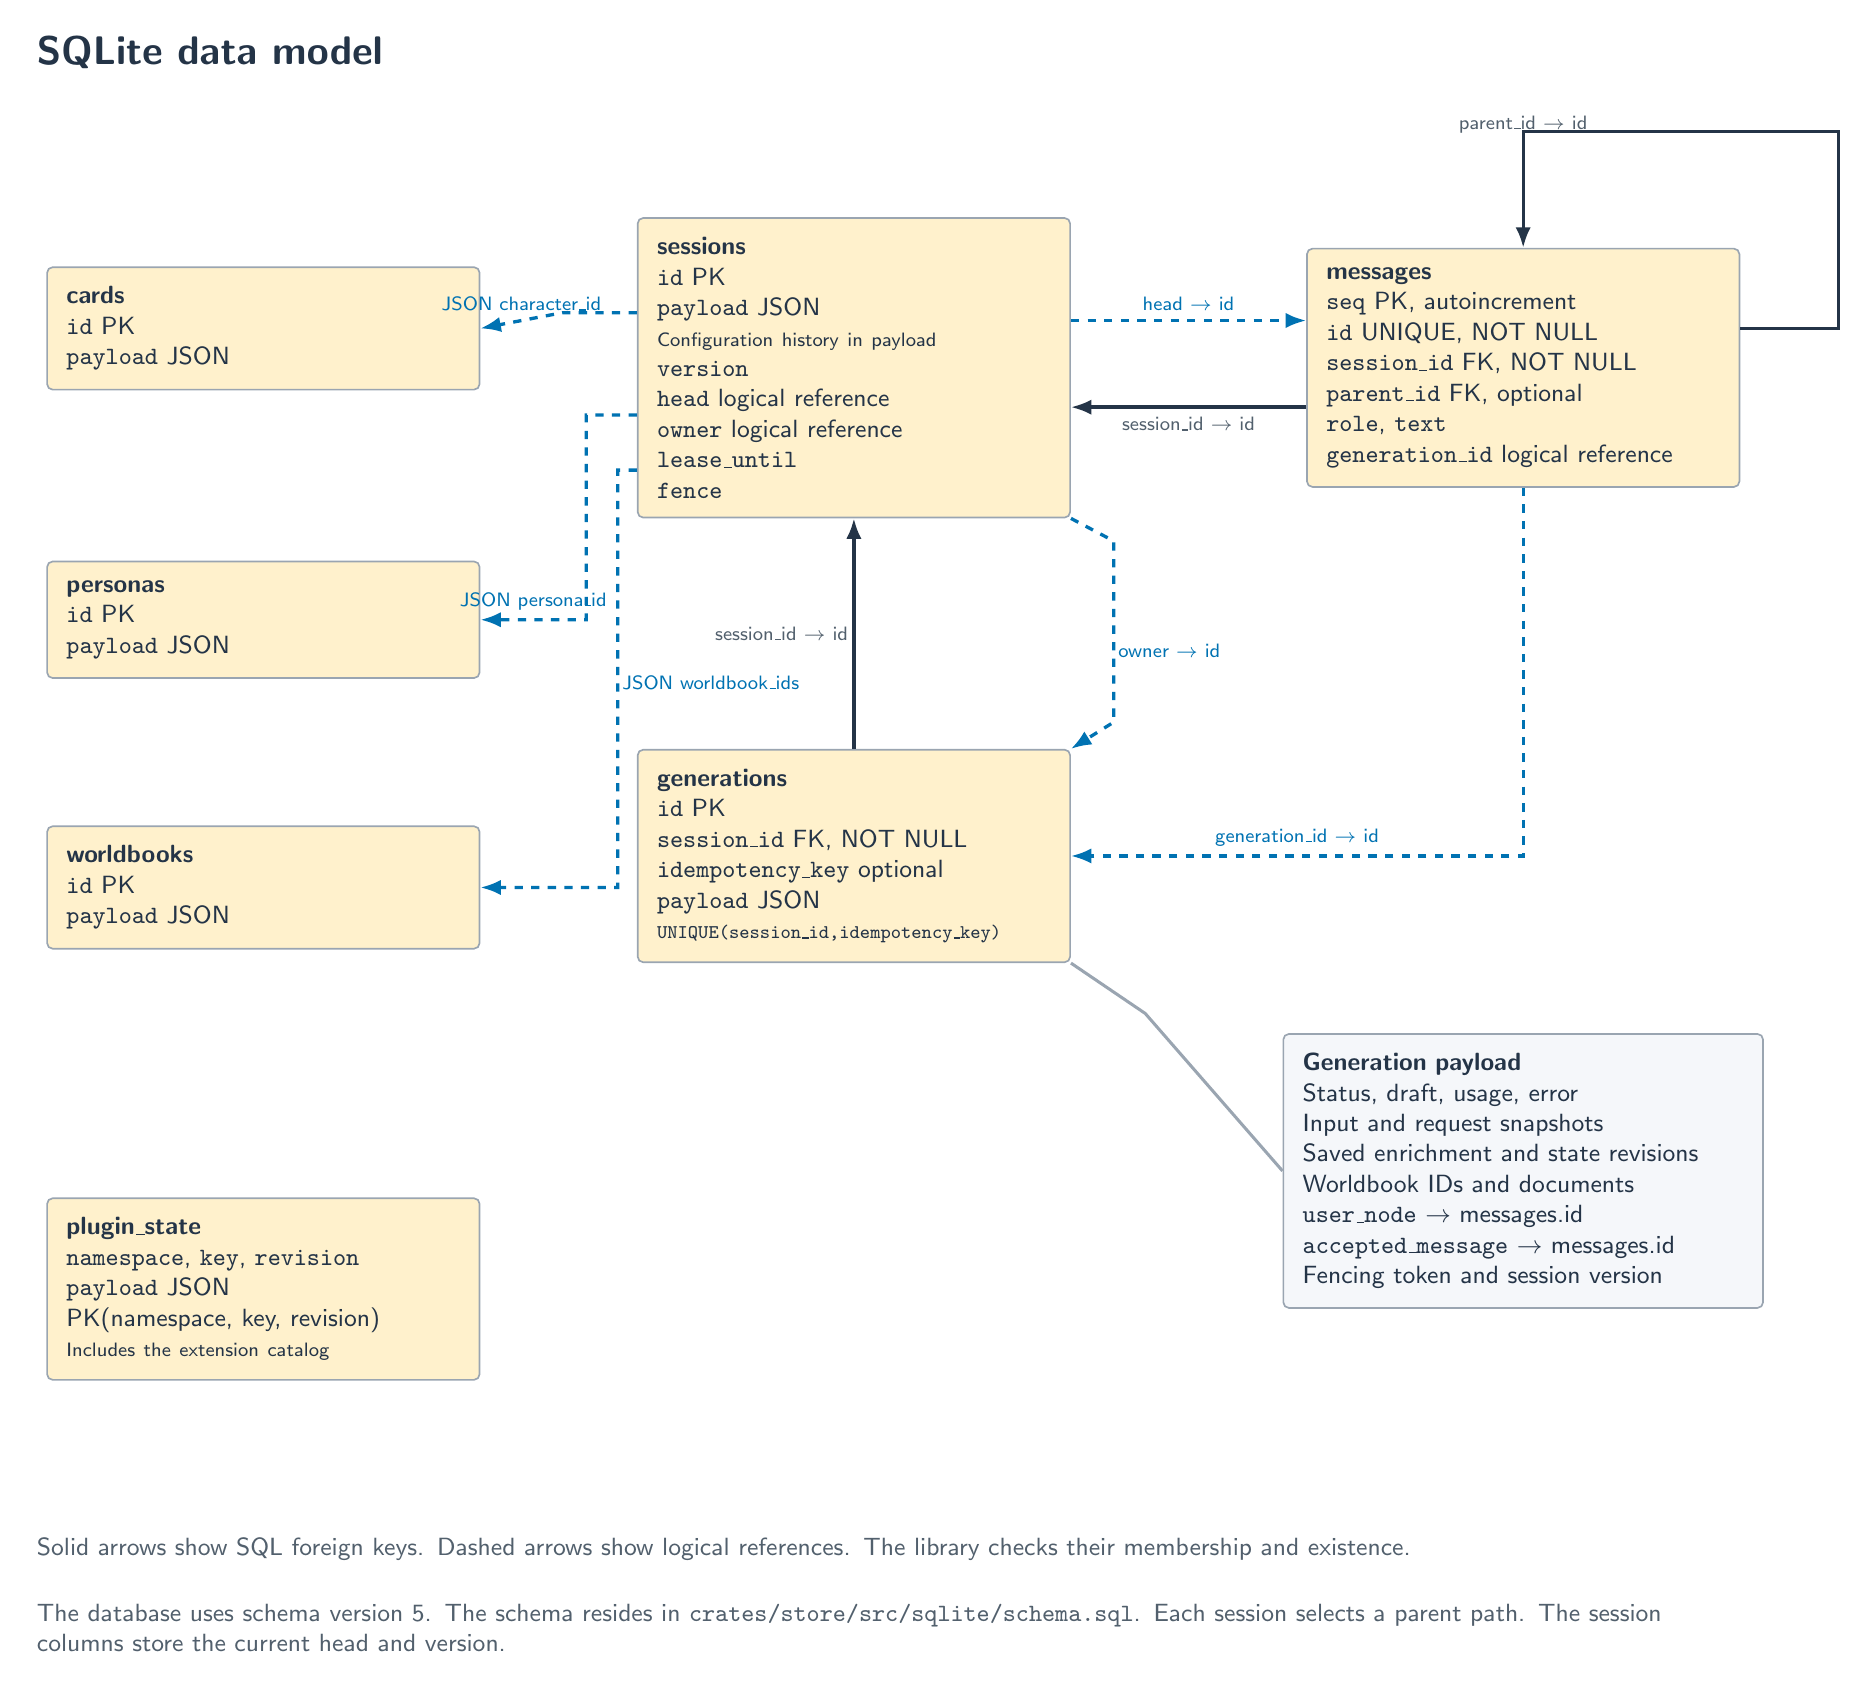
\begin{tikzpicture}[x=1cm,y=1cm]

\node[title] at (-1,15) {SQLite data model};
\node[table,fill=storefill] (cards) at (2,11.5) {\textbf{cards}\\\texttt{id} PK\\\texttt{payload} JSON};
\node[table,fill=storefill] (personas) at (2,7.8) {\textbf{personas}\\\texttt{id} PK\\\texttt{payload} JSON};
\node[table,fill=storefill] (sessions) at (9.5,11) {\textbf{sessions}\\\texttt{id} PK\\\texttt{payload} JSON\\{\scriptsize Configuration history in payload}\\\texttt{version}\\\texttt{head} logical reference\\\texttt{owner} logical reference\\\texttt{lease\_until}\\\texttt{fence}};
\node[table,fill=storefill] (messages) at (18,11) {\textbf{messages}\\\texttt{seq} PK, autoincrement\\\texttt{id} UNIQUE, NOT NULL\\\texttt{session\_id} FK, NOT NULL\\\texttt{parent\_id} FK, optional\\\texttt{role}, \texttt{text}\\\texttt{generation\_id} logical reference};
\node[table,fill=storefill] (generations) at (9.5,4.8) {\textbf{generations}\\\texttt{id} PK\\\texttt{session\_id} FK, NOT NULL\\\texttt{idempotency\_key} optional\\\texttt{payload} JSON\\{\scriptsize\texttt{UNIQUE(session\_id,idempotency\_key)}}};
\node[table,fill=storefill] (state) at (2,-0.7) {\textbf{plugin\_state}\\\texttt{namespace}, \texttt{key}, \texttt{revision}\\\texttt{payload} JSON\\PK(namespace, key, revision)\\{\scriptsize Includes the extension catalog}};
\node[table,fill=storefill] (worldbooks) at (2,4.4) {\textbf{worldbooks}\\\texttt{id} PK\\\texttt{payload} JSON};
\draw[fk] ([yshift=-5mm]messages.west) -- node[edge label,below] {session\_id $\to$ id} ([yshift=-5mm]sessions.east);
\draw[fk] (generations.north) -- node[edge label,left] {session\_id $\to$ id} (sessions.south);
\draw[fk] ([yshift=5mm]messages.east) -- (22,11.5) -- (22,14) -| node[edge label,pos=.55,above] {parent\_id $\to$ id} (messages.north);
\draw[logical] ([yshift=6mm]sessions.east) -- node[edge label,above,text=flowblue] {head $\to$ id} ([yshift=6mm]messages.west);
\draw[logical] (sessions.south east) -- (12.8,8.8) -- (12.8,6.5) -- (generations.north east);
\node[edge label,right,text=flowblue] at (12.8,7.4) {owner $\to$ id};
\draw[logical] (messages.south) -- (18,4.8) -- node[edge label,above,text=flowblue] {generation\_id $\to$ id} (generations.east);
\draw[logical] ([yshift=7mm]sessions.west) -- (5.8,11.7) -- node[edge label,above,text=flowblue] {JSON character\_id} (cards.east);
\draw[logical] ([yshift=-6mm]sessions.west) -- (6.1,10.4) |- node[edge label,pos=.75,above,text=flowblue] {JSON persona\_id} (personas.east);
\draw[logical] ([yshift=-13mm]sessions.west) -- (6.5,9.7) |- (worldbooks.east);
\node[edge label,right,text=flowblue] at (6.5,7.0) {JSON worldbook\_ids};
\node[table,fill=panel,text width=56mm] (payload) at (18,0.8) {\textbf{Generation payload}\\Status, draft, usage, error\\Input and request snapshots\\Saved enrichment and state revisions\\Worldbook IDs and documents\\\texttt{user\_node} $\to$ messages.id\\\texttt{accepted\_message} $\to$ messages.id\\Fencing token and session version};
\draw[relation] (generations.south east) -- (13.2,2.8) -- (payload.west);
\node[note,anchor=west,text width=210mm] at (-1,-4) {Solid arrows show SQL foreign keys. Dashed arrows show logical references. The library checks their membership and existence.};
\node[note,anchor=west,text width=210mm] at (-1,-5) {The database uses schema version 5. The schema resides in \texttt{crates/store/src/sqlite/schema.sql}. Each session selects a parent path. The session columns store the current head and version.};

\end{tikzpicture}
\end{document}
